\documentclass{article}
\usepackage[utf8]{inputenc}
\usepackage{pdfpages}

\title{Summarising Wireless Network Datasets}
\author{Charlotte Knight}
\date{September 2019}

\usepackage{biblatex}
\usepackage{graphicx}
\usepackage{longtable}
\usepackage{caption}
\usepackage{wrapfig}
\usepackage{latexsym}

\bibliography{references}

\begin{document}

\maketitle

\section*{Abstract}
There is lots of current research which requires data about the usage of wireless networks, however lots of time and effort must be spent separating out useful information from the huge amount of data now collected by wireless network monitoring. The amount of data sent over wireless networks will only continue growing in years to come. During this project a tool has been developed which enables relevant information for network mobility research to be extracted from multiple input sources and converted to a single, more manageable output. Processing stages in the tools data flow have been separated into individual components to enable easy expansion to new input formats in the future, with the current tool handling only tcpdump and syslog input. The minimum file size reduction seen on real tcpdump traces was found to be 99.992\%. The tool which has been developed has a quadratic dependency of execution time on the number of device-to-device associations in the input data. This dependency could become an issue if very large data sets need to be used with it.
\label{section:abst}
\newpage
\section*{Declaration}
I declare that the material submitted for assessment is my own work except where credit is explicitly given to others by citation or acknowledgement. This work was performed during the current academic year except where otherwise stated. 
The main text of this project report is 11,087 words long, including project specification and plan. 
In submitting this project report to the University of St Andrews, I give permission for it to be made available for use in accordance with the regulations of the University Library. I also give permission for the title and abstract to be published and for copies of the report to be made and supplied at cost to any bonafide library or research worker, and to be made available on the World Wide Web. I retain the copyright in this work.

\newpage
\tableofcontents
\newpage

\section{Introduction}
\label{section:intro}
%Need to re-write, much more detail needed
With such large quantities of wireless traffic now travelling through networks at ever increasing rates, processing of this data can be challenging. By introducing a summarisation step before any main processing the overall efficiency of information extraction from wireless network datasets may be increased. The aim of this project will be to create a summarised report from large datasets in order to enable more efficient onward processing of the data. This will mean using statistical approaches to maintain some identified information from the dataset while reducing the overall quantity of data that must be stored and processed. The output summaries created may utilise an existing format if my research can identify an appropriate one. My project will produce a command line application involving new approaches to summarisation to run over data collected in the CRAWDAD archives, the approach taken may (in this project or otherwise, dependent on time constraints) also be extended to work on datasets in real-time so as to eliminate the need for storing large datasets before summarisation.


\section{Context Survey}
\label{section:context}
    \subsection{CRAWDAD Usage}
    \label{section:useage}
    \subsubsection{Research}

When completing this research the focus has been on one particular dataset from the CRAWDAD archive, dartmouth/campus \cite{dartmouthcampus2009}. This dataset was chosen because it is one of the most popular datasets in the archive, having been cited by 374 papers at the time of writing \cite{aboutCrawdad2014}. The most frequently cited dataset however is cambridge/haggle, the reasoning for deciding not to focus on this instead is that the Cambridge dataset is comparatively small in size and would therefore benefit much less from the summarisation which this project hopes to provide.
\newline
The papers that have been selected for use in this research were chosen because they all cite the dartmouth/campus dataset. A Google Scholar \cite{googleScholar} online search was used to retrieve the most "relevant" papers which used the chosen dataset, from these results the ones which have been most often cited in other work were selected. This selection process found papers which are relevant in the research community. As there are different versions of the dataset the search had to be repeated three times, once using the 2009 dataset, once with the 2007 dataset, and once with the 2005 dataset. For each search the five most cited results have been used. Table \ref{usageTable} shows a summary of the type of information each paper needed to use from the dartmouth/campus dataset. Papers in which the dataset was referenced but ultimately has not been used have been excluded.

\small
\begin{longtable}{|p{3cm}|p{1.9cm}|p{1.7cm}|p{1.5cm}|p{1.9cm}|}
\cline{3-5}
\multicolumn{2}{}{} & \multicolumn{3}{|p{4.5cm}|}{Properties Needed} \\ \hline
Paper                                                & Topic                              & Device/AP Identification   & Time of Transmission  & Transmission Quality/Rate  \\ \hline
%308
Nextplace: a spatio-temporal prediction framework for pervasive systems, \citeauthor{Scellato2011}, \citeyear{Scellato2011}   & Mobility                           & x                          & x                     &                            \\ \hline
%191
Community-Aware Opportunistic Routing in Mobile Social Networks, \citeauthor{Xiao2014}, \citeyear{Xiao2014}           & Mobility                           & x                          & x                     &                            \\ \hline
%155
On nodal encounter patterns in wireless LAN traces, \citeauthor{Hsu2010}, \citeyear{Hsu2010}             & Mobility                           & x                          & x                     &                            \\ \hline
%140
Mobility models for systems evaluation, \citeauthor{Musolesi2009}, \citeyear{Musolesi2009}   & DTN                                & x                          & x                     &                            \\ \hline
%60
Large-Scale Synthetic Social Mobile Networks with SWIM, \citeauthor{Kosta2014}, \citeyear{Kosta2014}         & Mobility                           & x                          & x                     &                            \\ \hline
%27
WAVEFORM DESIGN AND NETWORK SELECTION IN WIDEBAND SMALL CELL NETWORKS, \citeauthor{Yang2014}, \citeyear{Yang2014}           & Mobility                           & x                          &                       & x                          \\ \hline
%18
MAGA: A Mobility-Aware Computation Offloading Decision for Distributed Mobile Cloud Computing, \citeauthor{Shi2018}, \citeyear{Shi2018}             & Mobility                           & x                          & x                     &                            \\ \hline
%18
Flow-Based Management For Energy Efficient Campus Networks, \citeauthor{Amokrane2015}, \citeyear{Amokrane2015}   & SDN                                & x                          &                       & x                          \\ \hline
%16
Human behavior and challenges of anonymizing WLAN traces, \citeauthor{Kumar2009}, \citeyear{Kumar2009}         & Anonymizing WLAN Traces            & x                          & x                     &                            \\ \hline
%15
Automatic profiling of network event sequences: algorithm and applications, \citeauthor{Meng2008}, \citeyear{Meng2008}           &Profiling of Network Event Sequences& x                          & x                     &                            \\ \hline
%13
Confidentiality of event data in policy-based monitoring, \citeauthor{Montanari2012}, \citeyear{Montanari2012} & Policy-Based Monitoring            & x                          &                       &                            \\ \hline
%12
Distribution of inter-contact time: An analysis-based on social relationships, \citeauthor{Wei2013}, \citeyear{Wei2013}             & Distribution of Inter-Contact Time & x                          & x                     &                            \\ \hline
%12
Coverage and Rate Analysis for Facilitating Machine-to-Machine Communication in LTE-A Networks Using Device-to-Device Communication, \citeauthor{Swain2017}, \citeyear{Swain2017}         & Machine-to-Machine Communication   & x                          & x                     &                            \\ \hline
%10
Balancing reliability and utilization in dynamic spectrum access, \citeauthor{Cao2012}, \citeyear{Cao2012}             & Dynamic Spectrum Access            & x                          & x                     &                            \\ \hline
%9
An Online Algorithm for Task Offloading in Heterogeneous Mobile Clouds, \citeauthor{Zhou2018}, \citeyear{Zhou2018}           & Offloading                         & x                          & x                     &                            \\ \hline
%6
State-of-the-Art Routing Protocols for Delay Tolerant Networks, \citeauthor{Feng2012}, \citeyear{Feng2012}          & DTN                                 & x                          &                       & x                          \\ \hline

\captionsetup{width=\textwidth}
\caption{Table of the properties of CRAWDAD dartmouth/campus data used in various research projects in which it was cited. Papers are ordered by the number of other papers they have been cited by, with the most cited at the top.}
\label{usageTable}
\end{longtable}

\subsubsection{Summary of Results}
The usage of the Dartmouth University CRAWDAD dataset is primarily regarding network mobility and social interaction/encounters. As such, the most often needed information seems to be identifiers for both mobile devices and access points, and the times of connections.
I found that the majority of the papers I looked at used the movement \cite{dartmouthcampus2009movement} or syslog \cite{dartmouthcampus2009syslog} tracesets as these are most tailored towards mobility research. 

There are also some less frequent topics of research such as software defined networking and delay tolerant networking using the dartmouth/campus dataset. These uses seem to require a wider variety of information from the data, however these instances are much less frequent than those mentioned above. these less common cases are the only ones which mention bandwidth and quality of connection.


    
    \subsection{Formats}
    \label{section:formats}
    \subsection{Existing Formats for Aggregation of Network Traces in Mobility Research}

A lack of published information on the intermediate formats used while analysing network traces for mobility research has been found during this research. This is likely due to the encounter data not being the final outcome of the research taking place and therefore not being considered important enough to write up.

Through varied searches of DTN, Mobility, and SDN research I have found only two examples of well documented formats for storing data on device encounters. The first of these, The ONE Simulator \cite{Keranen2009}, uses several reporting options to store device encounter data. The other documented format (from \cite{Thakur2012}) that was found was an association matrix. These two sources and and analysis of the information found in them is set out in the following section of this report.

\subsubsection{The ONE Simulator \cite{Keranen2009}}
The ONE is a simulator which generates data intended to mimic a network of mobile nodes. It then reports this data using various reporting modules, three of these modules focus on data regarding encounters between devices.

The first and most simple of these reports contains information about the dispersion of the total number of encounters experienced by the nodes in the network. It consists of two fields, one containing the number of encounters, and the other containing the count of nodes that have experienced that number of encounters. This contains no information relating to the unique nodes between which the encounters occur, or any temporal information such as duration of the encounters. 

The second format provides information on the uniqueness of the encounters recorded, but loses detail about the total number of encounters in the dataset. This format also contains two data fields, one containing the values from 0 to 1000; representing promilles. The second field contains the number of unique pairs encountering with frequency withing the corresponding promille. This has a benefit of being almost static in size as the number of nodes int he system increases. 

The final report format from the ONE simulation which has been looked at is a combination of the two previously discussed reports. It has three fields; the first contains an identifier for each node, the second contains the total number of encounters that the node has had, and the third contains the number of unique nodes with which it has had an encounter. This still does not uniquely identify both devices in an encounter, nor does it provide and detail about the duration of the encounters.

\subsubsection{Association Matrices}
\citeauthor{Thakur2012} use an association matrix to record the percentage of time each node spends in an encounter with each other node. A matrix is created for each node, each column in the matrix corresponds to the other endpoint of the encounter, and each row corresponds to a time interval. The entry in each cell represents the percentage of the time interval spent in an encounter with the columns node. This format contains the most information out of all those discussed here, however also takes more space. The space taken will increase at with the square of the number of nodes.

\begin{table}
\small
\begin{tabular}{|p{5.5cm}|p{1.5cm}|p{1.5cm}|p{1.5cm}|}
\cline{3-4}
\multicolumn{1}{}{} & \multicolumn{3}{|p{4.5cm}|}{Level of Detail (Complete, Most, Some, or None)} \\ \hline
 Format&Endpoints&Duration&Frequency\\ \hline
 TotalEncountersReport - The ONE \cite{Keranen2009}&Some&None&Complete \\ \hline
 UniqueEncountersReport - The ONE \cite{Keranen2009}&Some&None&Most \\ \hline
 EncountersVsUniqueEncounters - The ONE \cite{Keranen2009}&Most&None&Complete \\ \hline
 Association Matrix \cite{Thakur2012}&Complete&Some&Some \\ \hline
 
\end{tabular}
\caption{Table of existing formats for storing data about device encounters and the level of detail they contain regarding the unique endpoints and length/frequency of the encounters.}
\label{formatTable}
\end{table}


\subsection{Summary of Findings}
A very brief summary of the detail contained within each of the formats discussed above is given in Table \ref{formatTable}. Despite association matrices storing the most useful information, the polynomial increase in size with the number of mobile nodes makes using them potentially ineffective in the context of this project. The aim is to summarize a large amount of data into a smaller, easier to process format. In many cases association matrices would decrease the size of the data, but by a dramatically lesser amount than the other formats discussed here. Additionally it would be possible for the association matrix format to increase the quantity of data; for instance if $N$ nodes had $< N$ encounters each then the association matrix for each node would include at least one redundant column. The final reporting format discussed under the ONE simulation - EncountersVsUniqueEncounters - avoids this polynomial growth, with its size increasing only linearly with the number of mobile nodes in the network. It provides less complete information regarding the unique par of nodes between which the encounter occurred, there would however be no way to preserve this information while avoiding at least $N^{2}$ growth in size.

It seems that the most complete format of those discussed in which to store encounter data while also guaranteeing a reduction in the quantity of data stored would be the EncountersVsUniqueEncounters report format. This format could also be easily modified to add additional fields such as statistics regarding encounter duration. Any additional fields would need to be carefully considered and justified in order to keep the data quantity reduction as high as possible.

\section{Requirements Specification}
\label{section:req}
In order of priority the requirements of this project have been listed below. These are the same requirements as set out in the DOER document submitted at the beginning of this project, and have been described in greater detail here. Each of these requirements can be implemented separately from one another, and with the completion of all high priority requirements a working product will be completed. The high priority requirements combine to describe a minimum viable product to meet the overreaching aims of this project. \\
Implementation of the medium and low priority requirements will complete a more versatile system which could be applied to datasets with a wider variety of sizes and formats.\\
All of the requirements set out here are functional requirements, in that they describe features to be implemented in order to produce a high quality summarisation tool.

\subsection{High Priority}
\begin{itemize}
    \item Reduce the quantity of data from the original dataset while maintaining any information identified as useful during research into how CRAWDAD datasets are used.
    \begin{itemize}
        \item During the context survey it was found that the most used information from these datasets was the encounters between different devices. Mobile node encounters (including the nodes involved and duration) will need to be included in the summaries for this requirement to be met. 
        \item It is important that the total quantity of data is reduced in the summary compared to the original dataset. For this requirement to be met it should be shown that the output is guaranteed to contain less data than the input.
    \end{itemize}
    \item Produce summaries of the initial datasets that can be processed more efficiently than the original data.
    \begin{itemize}
        \item In order to meet this objective it is necessary for the summary format to be as simple as possible. Superfluous information and complex file types will need to be avoided. 
    \end{itemize}
    \item Use a commonly found format to output my summaries and justify why this format is appropriate in context.
    \begin{itemize}
        \item In section 7 (Design) a complete output format will be specified and justification given based on the research in section 3.2.
        \item Specification of the output summary format should include the file type that will be used, the fields that will be included, and the variable types that will be used. All of these decisions will need to be supported by relevant and reliable research.
    \end{itemize}
\end{itemize}

\subsection{Medium Priority}
\begin{itemize}
    \item Allow multiple summaries to be merged (this may allow extension into distributed processing).
    \begin{itemize}
        \item This should allow two summaries which have been output by the minimum viable product to be given as arguments at run time and combined into a single summary.
        \item The output of this will use the same format as the input summaries, as if created by running the basic program on the combined network traces. 
    \end{itemize}
    \item Summarise at least two different formats of input data to create a standard output summary.
    \begin{itemize}
        \item The system will support summarising more than one input format, but the input format should be specified at run time.
        \item Whichever format the input takes the same output format should be produced. 
    \end{itemize}
    \item Allow a summary to be updated by the addition of a single data entry (this may allow extension into real-time processing).
    \begin{itemize}
        \item This requirement will be met if a summary can have added to it a single item of data (the exact definition of which will depend on the input format of the data, for instance a single data packet transfer in a tcpdump trace). With the resulting summary being identical to the summary which would have resulted from an initial input which included the new data entry.
    \end{itemize}
\end{itemize}

\subsection{Low Priority}
\begin{itemize}
    \item Process datasets with an unknown input format.
    \begin{itemize}
        \item The format of the input data should not need to be specified at run time.
        \item Multiple input formats should be accepted and and the system should be able to differentiate between them in order to process each correctly.
    \end{itemize}
    \item Identify and report if a specific summary is likely to be unrepresentative of the input dataset due to aspects such as missing data or bias.
    \begin{itemize}
        \item Depending on the information included in the summary, how representative it is may be effected for various reasons. Due to this it is important that any information used to determine whether a summary is unrepresentative is justified.
    \end{itemize}
\end{itemize}

\section{Software Engineering Process}
\label{section:proc}
%Time plan
During this project several separate development cycles were completed, each with a different end goal. Each cycle began with a research and planning phase which then lead to a implementation and testing phase. Testing was done continuously during the implementation of features, with additional performance testing done at the end of each implementation phase once all new features had been added.
Each week throughout the project a selection of tasks was made. At time flexibility was needed as some tasks were expected to take more than one week to complete. In such cases tasks were selected multiple weeks in a row.\\\\
As a final stage in each development cycle the product is evaluated against the requirements of this project. This gives a starting point for the next cycle, requirements which are fully met do not need to be implemented again in the next cycle, but still need to be given consideration to ensure future changes do not compromise them. \\\\
Throughout this project the school's Mercurial system has been used for version control. The Mercurial repository was use not only for the source code of the the summarisation tool but also to enable me to keep track of my own progress through weekly logging of the tasks which were completed and any issues that were encountered. By keeping track of past performance future weeks workloads were able to be more efficiently and realistically planned.S
\subsection{Development Cycle One: MVP}
The first development cycle was intended to be completed before the start of the second semester and to produce a fully working, well tested MVP which met all the high priority objectives set out in section 4 of this report.  
    %Research
    \subsubsection{Research and Planning}
    The first few weeks of this cycle were spent researching other work in the area, and completing the context survey as detailed in section three of this report. Then, using the findings from the research, the intended output format was specified. An outline for the stages needed during the processing of the data was decided and appropriate languages and libraries for each stage were decided on.
    %Development cycle 1 (MVP)
    \subsubsection{Implementation and Testing}
    Features that were implemented during this cycle were:
    \begin{itemize}
        \item The ability to take tcpdump output as input
        \item Extraction of encounters from input data into a simple CSV format 
        \item A simple command line interface allowing and input directory to be specified
        \item A BASH script tying together the three stages of the MVP's data flow
    \end{itemize}
    Once these features were implemented through tests were done using the CRAWDAD dartmouth data. The output was considered to be reasonable by inspection of the number of access points detected by the summarisation tool. In addition the length of associations and encounters were checked to make sure they were realistic in the context of the building in which the data was collected. Complete accuracy was difficult to ensure since there is not existing encounter data to compare this output to.\\\\
    After completing some testing of the time efficiency of the data processing showed that this initial implementation was unreasonably slow under certain conditions. Specifically when high numbers of access points were used, the matching of associations into encounters took a long time to run. Once five access points were detected the process would take several hours to run, while the same length of input with only two distinct access points would complete processing in around twenty minutes. Speeding this up is something considered in the next cycle.
    \subsubsection{Evaluation Against Requirements}
    The product developed by the end of this cycle satisfies the first two of the high priority requirements identified in section 4. The quantity of data is significantly less in the output of the product than the input. Research was done which identified encounters between devices as the most useful information in the data, so this information was kept in the output. The third high priority requirement was only partially met at this stage; the CSV format used for output has several benefits (such as its simplicity and flexibility) however no evidence has been found to support its use in the context to encounter traces in existing mobility research.   
\subsection{Development Cycle Two: Extending Capabilities}
In this second cycle the aim was to find a more justifiable output format, to improve the time efficiency of the existing code, and to add features which extend the functionality of the product. The medium priority requirements in section 4 should be considered while adding functionality.
    %Research
    \subsubsection{Research and Planning}
    The research in this cycle was mainly technical topics. A better understanding of the MatLab language was needed in order to write more efficient code, and so further research into the strengths and weaknesses of the language was undertaken. The ONE simulator was also further researched and how the output of this project could be altered to be compatible with it.
    %Development cycle 2 (Extending)
    \subsubsection{Implementation and Testing}
    Updated and improved functionality:
    \begin{itemize}
        \item The speed dependency of the processing on the number of access points was reduced from a quadratic relationship to a linear one
        %\item The output of the product was altered to be compatible with the ONE simulator [TODO!]
    \end{itemize}
    These additional features were added:
    \begin{itemize}
        \item Capability to parse syslog files in addition to tcpdump
        %\item Multiple summaries can be merged to create a single output of similar format [TODO!]
        %\item A summary may now be updated by a single data entry [TODO, possibly won't get time]
    \end{itemize}
    By using appropriate data structure in MatLab the languages efficient referencing and searching was able to be used. This greatly reduced processing time when the intermediate associations data needs to be matched against known access points. It was this efficiency of MatLab that made it a justifiable choice for implementing the transformation from associations to encounters, however an inefficient method of looping through associations had mistakenly been used in the first implementation.
    \subsubsection{Evaluation Against Requirements}
    During this development cycle one additional medium priority requirement has been met (ability to summarise multiple known input formats). In addition to this the performance of the summarisation tool has been improved, and progress has been made toward using a more suitable output format which will be compatible with the ONE simulator.
    
%Ongoing change
    %

%Testing
    %



\section{Ethics}
\label{section:ethi}
The potential ethical risk associated with this project is low since there will be no contact with participants (such as interviews or questionnaires), and no personally identifiable data is expected to be used. 
Datasets of wireless network activity downloaded from the CRAWDAD archive will be used in this project. The datasets which are to be summarised in this project are sanitised, meaning that details such as IP and MAC addresses have been changed to obscure the identities of the network users. Despite this there is a minor risk that identifying information may be accidentally extracted during the processing of this data.
If any personally identifiable data is extracted it will be removed from any devices which it may have been stored on and the code which caused the mistake will be reviewed to prevent it from happening again. A full ethics application has been made for this project and has been given the approval code CS14642. The ethical application form has been appended to this document in Appendix \ref{section:ethics_append}.

\section{Design}
\label{section:des}
\subsection{Data Flow}

\subsubsection{Input and Processing}
Multiple formats can be processed using the command line tool that has been developed during this project. Processing multiple input formats allows for  Initially only TCPdump was considered since it is the format with the most redundant information, and therefore on which summarisation would give the greatest benefit. The tool took input in the form of binary PCAP files, however this was then extended to allow syslog formats to be used as input. The output produced is in an identical format regardless of the input type. Using a consistent output format regardless of the input format is important as it means that researchers can treat data collected from multiple sources similarly. Data flow for the two input types is nearly identical and is detailed in figure \ref{fig:df_dia}.\newline
\begin{figure}[h]
    \centering
    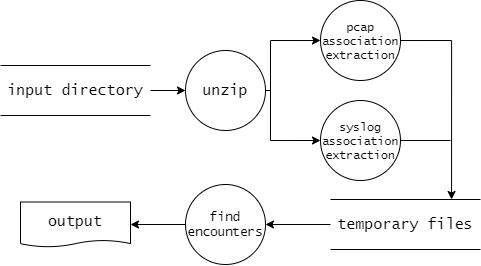
\includegraphics[width=0.7\textwidth]{df_diagram.png}
    \caption{This figure shows the flow of data through the system, including temporary file stores and input/output to each processing stage.}
    \label{fig:df_dia}
\end{figure}

The first stage of processing is to extract associations between devices and access points from the raw input. These associations will later be compared with each other to determine encounters between devices, these comparisons are expensive and so it is important that as much information as possible is removed before they are made. The intermediate format used to store association information is  a comma separated value file. MatLab is used in the second stage of processing and has a very good interface for reading character delimited text files such as CSV format. The intermediate format has fields of source id, destination id, start time, end time, and AP flag. The AP flag is set to 1 only if the destination address of the association can be identified as an access point. Methods used to identify access points are discussed later in this report.

TCPdump output PCAP files are very strictly structured. This allows for them to be processed without any additional information from the user. However the initial parsing is expensive with respect to time since so much information is contained within them. In comparison to this, syslog files are relatively quick to parse for associations. Syslog formats vary according to the preferences of the network administrator, so the user must include a configuration file to specify the format used. Details such as defining features of association end points and the format of device identification values need to be given to the tool before it can extract associations. A timestamp in seconds must be included for key lines in the syslog file for it to be parsed by this tool successfully. The expected format of a configuration file for use with syslog is detailed in figure \ref{fig:JSON_config}. Several configuration file formats were considered for use here, with final choice being to use a YAML structure. YAML allows more complex nested structures than other similar formats while staying more human readable than alternatives such as JSON.

\begin{figure}[h]
    \centering
    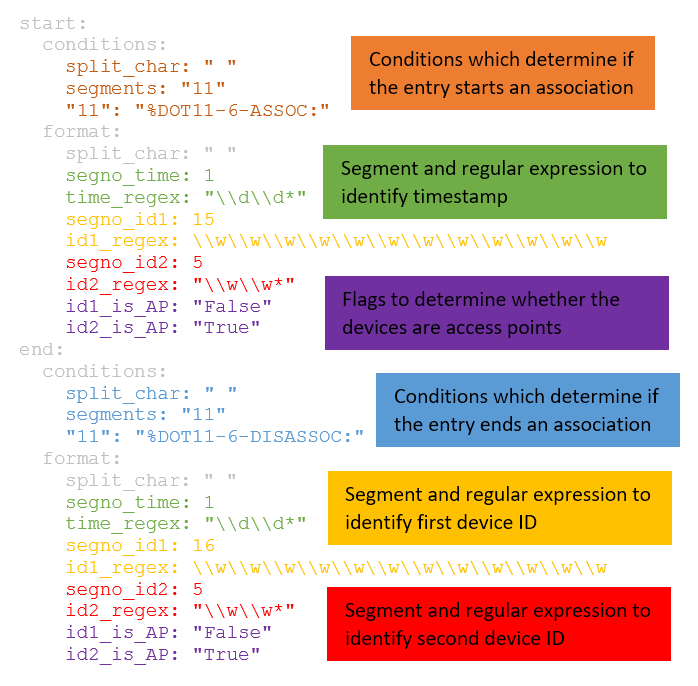
\includegraphics[width=0.9\textwidth]{conf.png}
    \caption{This figure shows a YAML configuration file used for the processing of the dartmouth/campus Cisco syslog files. The fields have been colour coded for readability and descriptions of the fields have been given. The colour does not reflect any formatting of the actual configuration file. It should be noted that although the regular expressions are the same in both the start and end sections of the configuration file shown, this is not a requirement.}
    \label{fig:JSON_config}
\end{figure}

An example of how the configuration shown in figure \ref{fig:JSON_config} is applied to a syslog file \cite{dartmouthcampus2009syslog} is shown in figure \ref{fig:cisco_syslog} using the same colour scheme. This is a simple example and more complex configurations may include multiple start and/or end blocks (allowing multiple differently structures lines to be recognised as the start or end of an association). Multiple conditions could be used within each start and/or end block, all of these would then need to be satisfied for the line to be recognised as matching that block. 
\begin{figure}[h]
    \centering
    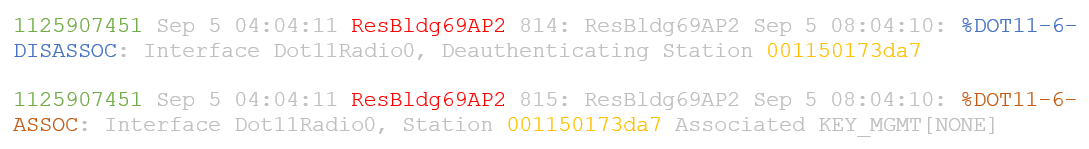
\includegraphics[width=\textwidth]{cisco_coloured.png}
    \caption{This figure shows a two line extract of the dartmouth/campus Cisco syslog files \cite{dartmouthcampus2009syslog}. The information used by the summarisation tool is colour coded matching the parts of figure \ref{fig:JSON_config} which identify it. The first line shown matches the conditions for the end of an association, and the second line matches the conditions for the beginning of an association.}
    \label{fig:cisco_syslog}
\end{figure}
\newline
Tying together the components of this data flow is a BASH script, this can be configured using flags at run time. The BASH script allows for data to be piped between some processing elements, and for temporary files to be shared between processing stages. Temporary files are used for storing associations in the intermediate stages, these files are then read by the MatLab script which compares associations to find encounters. A final output file is then given either as a comma separated values file or a ONE simulator events trace, and all temporary files are cleaned up. 
% Optional levels of abstraction??

% explain fields chosen
%   - how is encounter data used in external studies?
% Data flow diagrams
% BASH scripting

\subsubsection{Summary Output}
The final output can be given in one of two formats, the first (default output) specifies the endpoints of encounters, the average time of encounters between the given end points, and the number of encounters found between the given end points. Only one entry in the CSV file is present for each unordered pair of end points. A small section of an output summary is shown in figure \ref{fig:output}, it has been colour coded for ease of reading.\newline
\begin{figure}[h]
    \centering
    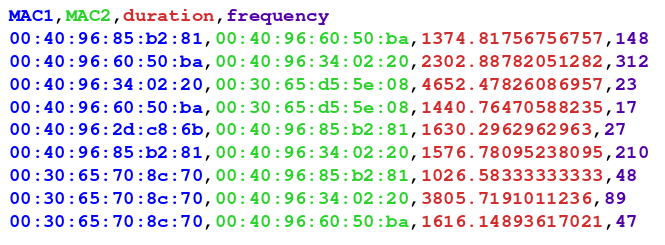
\includegraphics[width=0.8\textwidth]{Output_Example_Coloured.png}
    \caption{This figure shows a small section of an output file produced by the summarisation tool developed during this project. The columns have been colour coded for readability, but this does not reflect any formatting of the output CSV.}
    \label{fig:output}
\end{figure}

The data sets which I am using in this project have in the past frequently been used for research into mobility and encounter patterns between users \cite{Scellato2011} \cite{Xiao2014} \cite{Hsu2010} \cite{Musolesi2009} \cite{Kosta2014} \cite{Kumar2009} \cite{Wei2013}. To maximise the usefulness of this project it is intended that the output from this  summarisation tool will be able to help in identifying whether a dataset is appropriate for use in mobility research, and to provide a standard format between multiple input formats which can be used for onward processing.

The second format which can be used for output is an events file compatible for use with the ONE simulator \cite{Keranen2009}. The ONE simulator is a commonly used tool in mobility research, it is a simulation environment which can show interactions in a network using its GUI, or produce a variety of reports (including some regarding node mobility). Real-world event data can be used in simulations using the ONE simulator. Additional input may be necessary in some applications, such as geographical information about the environment in which the network event were collected, or connection speeds and ranges. This additional information is out of the scope of this project, in the examples given in this document the minimum additional information is used for simulations (mostly settings are maintained as they were in the default settings configuration from the installation source directory). Figure \ref{fig:events_out} shows an extract of this event trace output.
\begin{figure}[h]
    \centerline{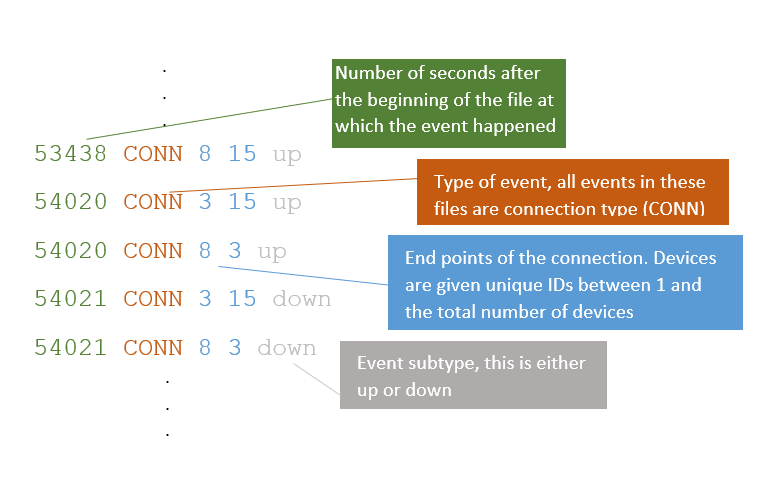
\includegraphics[width=0.9\textwidth]{events_output.png}}
    \caption{This figure shows a small section of an output file produced by the summarisation tool developed during this project. Each field has been colour coded and explained alongside the extract.Only events of type `CONN' are recorded in the events traces output by this summarisation tool. `CONN' events can have subtype `up' for the beginning of a connection (or in the terms used in this paper, the beginning of an association) or `down' for the end of a connection.}
    \label{fig:events_out}
\end{figure}

A variant on the events file format which maintains the original timestamps and device identifications is also provided, the use of which is discussed in section \ref{section:merge}.

\subsection{Associations} 

\begin{figure}[h]
    \centerline{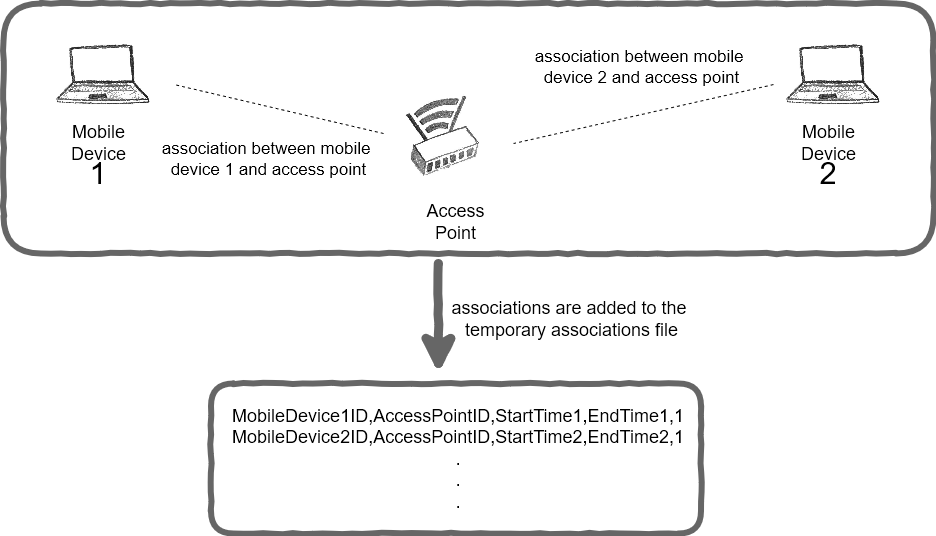
\includegraphics[width=1.2\textwidth]{hardware_to_assoc.png}}
    \caption{This diagram shows a high level representation of two associations and the corresponding network connections which would cause them. If these two associations were active during the same period of time, an encounter would exist between the two mobile devices.}
    \label{fig:high_level_dia}
\end{figure}
In this project two identifiable devices are considered to be associated with each other for any period of time during which they are exchanging data, a graphical representation of this is shown in figure \ref{fig:high_level_dia}. Due to the definition of encounters (explained in more detail is section \ref{section:encounters}) in this context only associations between one mobile node and one access point are relevant. In addition a device might only be identified as an access point after several packets have been exchanged with it, it is therefore important that all associations are detected and recorded until a full list of access points is available.
%(what? why?)
\subsubsection{Identifying Access Points}
Access points need to be determined as only the associations with access points are needed in the later stage of this processing. Access points may be identified from tcpdump traces by reading the flags in the TCP header of the packets sent to them. The SYN control flag of TCP packets is checked, when it is set to true the destination of the packet can be determined to be an access point. Once a packet is identified as an access point a flag is set by it in the intermediate temporary associations CSV file. This flag is used in later processing to remove all irrelevant associations from the data and to create a record of all detected access points in the network. By removing irrelevant associations the time efficiency of the summarisation is increased, as fewer comparisons have to be made in order to identify all encounters. A full list of access points must be completed before associations are matched into encounters; if the access point list was built as the associations were searched some encounters early in the data may be missed.\\\\
This method of detecting access points means that access points which do not exchange TCP data with any mobile nodes will not be detected, and therefore encounters which occur through them will not be recorded. It is unlikely for a network trace running over a significant period of time that an access point will associate with multiple devices and yet not transfer any TCP packets with them, this means that any access points not detected by this method are extremely unlikely to have facilitated any encounters.\\\\
When parsing syslog files the location and format of the access points identifications should be specified in the configuration file. As all association and disassociation messages in a syslog file should contain an access point, all lines in the intermediate temporary associations CSV file created from a syslog input will be set as true. Despite this potentially seeming to be a waste of time to set all flags to true, it is necessary to maintain the intermediate format so that the next stage of processing can be completed using the same method regardless of initial input format.
Some input files showed hundreds of access points being detected. This is likely due to each physical access point having many separate MAC addresses with which it will communicate. There is no way to identify which addresses correspond to the same physical access point without a record to match them against. Since such a record is not available for the CRAWDAD dartmouth/campus data (and likely wouldn't be immediately available for most network traces someone might want to use with this summarisation tool) the decision has been made to only consider an encounter to have taken place is both mobile devices are connected to the same access point MAC address. This is similar to saying that each MAC address being used by a physical access point has been considered as a separate device.
\subsubsection{Initiation} 
% (what? why?)
A design decision needed to be made regarding the conditions that would specify the beginning of an association between two devices. This is an important part of the design of this system since it defines the meaning of an association, and therefore the meaning of an encounter in the final output of the system.\\\\
Identifying association request packets could be used as a method of identifying the beginning of associations. However it has been found during development that often two devices are in contact and transmit data between themselves without ever sending an association request packet. Since an association is open during the period of time which two devices are communicating, a simplistic way of finding the start of an association may be the timestamp of the first packet transmitted between two identifiable devices.\\\\
It was decided that with a tcpdump input, the initiation of an association would be triggered by a packet being transmitted between two devices which do not currently have an ongoing association. While an association is ongoing a transmission between the endpoints will not trigger a new association. If only one packet is transmitted between the endpoints within the timeout period it is not considered as an association. This is because it may have been a message sent to an unavailable destination, and in such a situation no contact is made between the source and destination devices.\\\\
Syslog files may have varying structures so a way to identify the location of key information within the file is needed. Therefore, when a syslog file is used as input the configuration file should contain conditions for a message to define the start of an association. These condition will have to be checked against each line in the syslog file to find the beginning of each association. The endpoints of the association should also have their identifications location and format within the line described in the configuration file. In the case that a configuration file specifies conditions which are ambiguous (for instance causing multiple matches for a devices identification within the line) or too strict (for instance not finding any association start messages or not being able to identify any device identifications which match the conditions given int he configuration file) then the user should be warned. Such a case my occur if the configuration file has been mistyped or the wrong configuration file is being used, however it could also be triggered in a case with unexpected data such as no associations occurring. By warning the user it gives them the opportunity to update the configuration file if necessary, but will not prevent the tool being run using a configuration file which triggers the warning.
% options
% decision

\subsubsection{End of Association} 
% (what? why?)
In some cases a specific message or packet type may be found which determines that a device has moved out of range of an access point. This would mean that the association between that device and access point has come to an end. However, in the pcap traces which I have been focusing on it seems common that the end of an association is not explicitly signalled in the trace. In these cases another method of detecting an appropriate time for ending an association is needed. \\\\
Research into work already done with the CRAWDAD data \cite{kotz2002} \cite{henderson2004} shows that a timeout of thirty minutes has previously been considered to be adequate for determining the end of a session, leading to a deauthentication of the device. This timeout length will therefore be use in this project to catch the end of associations when no explicit disassociation is found. 
When working with a tcpdump input, if no packets are transmitted between two associated devices for a thirty minute period the end of the association will be recorded using the timestamp of the most recent packet transmitted between them. When a syslog input is being used, conditions which identify a message showing the end of an association should be specified in the configuration file similarly to how they were specified for the beginning of an association.
% research
% decision
% alternatives? why not?

\subsection{Encounters} 
% (what? why?)
\label{section:encounters}
\begin{figure}[h]
    \centerline{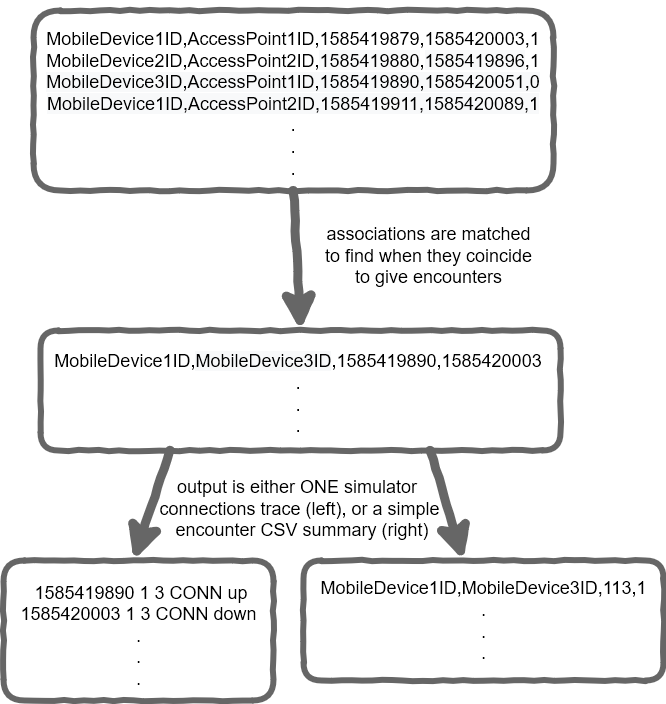
\includegraphics[width=0.8\textwidth]{assoc_to_enc.png}}
    \caption{This diagram shows a example of how associations may be matched together to find encounters, and how the encounters may then be output in both available formats. Timestamps here are left as Unix epoch times since only a fragment of data is shown. In actuality times would be converted to an offset (in seconds) from the beginning of the first encounter found.}
    \label{fig:assoc_to_enc}
\end{figure}
Two devices are said to encounter each other when they are within communication ranger, encounters in this project have a resolution of seconds, but can last as long as the tcpdump or syslog trace records traffic for. Devices are assumed to be in transmission range of each other for the duration of time when they are associated with the same access point. Encounters between devices are considered to begin at the earliest time where both devices are connected to the same access point, and to end as soon as one of the two devices disassociates from the access point. An example of how an encounter would be found from a set of associations is shown in figure \ref{fig:assoc_to_enc}. To find details of an encounter it is necessary to know which device identifications belong to access points, as these will act to facilitate encounters rather than being the end points. The associations will need to be matched together by considering the time overlap in the case that they both use the same access point.\\\\
It is likely that these matches will need to be found in a large set of associations, over a long time period, and many access points. It will therefore be important for the implementation of this to be efficient. As previously mentioned, to maximise efficiency in this stage of processing all associations which definitely do not contribute to an encounter need to be eliminated from the data as soon as possible. This is achieved by removing all associations which do not include an access point as one end point as soon as a full list of access points has been identified.
% Encounters from associations
\subsection{Merging Summaries}
\label{section:merge}
In addition to the main summarisation of data, this tool also allows for the merging of multiple summaries into a single file of the same structure. By using the `merge' command when running the tool a directory of `.txt' or `.csv' files can be merged together. When encounters summaries (those of structure seen in figure \ref{fig:output}) are merged the output data is the same as if all of the initial network traces had been summarised together to begin with. However, the events output format (as seen in figure \ref{fig:events_out}) discards the real timestamps on the events and the real device identifiers. In the events format the time is seen relative to the beginning of the file and the identifiers are changed to be numerical (1 to the number of mobile devices). Due to these loses of information the event format output cannot be merged as is, however a summary output format is provided (selected by use of `events\_maintain\_identifiers' with the -t flag) which does not replace the device identifiers or timestamps, and is therefore friendly to the merging. When merging events files the output will be given with relative timestamps and numerical device identifications, the original values will not be kept after the merge.

The input directory (specified using the -i flag) should only contain one format of summary, if a mixture of encounters summaries and events traces is present then the tool will exit without producing the requested output file and will display an error to the user. If `.txt' or `.csv' files which are not in either summary output format are found in the input directory the tool will also display an error and exit without producing an output file.\\\\
The value of this feature is mainly due to the quadratic execution time at increasing association numbers (as discussed in section \ref{section:impl_stage3}). When a large input file is summarised it may be split into smaller input files and the resulting summaries merged back together resulting in a lower execution time for sufficiently high numbers of associations. For an input of size $N$ split into chunks of size $n$, the quadratic increase in time will be dependent on $n$, and a linear slow down is expected with respect to $N$. However, a faster execution time will only be observed in very large files due to the time taken to complete the merge, and the initialisation time needed for each chunk of processing. Associations would also be split at the boundaries of each input chunk, this effect may be minimised by choosing to split the input at times where the network is expected to be quietest.

The ability to merge summaries after processing sections of the input separately could lead into a distributed approach to handling large inputs, however such a distributed system has not been developed during this project. A system for deciding where to split files for maximum efficiency would need to be considered, as well as a method of splitting files which wouldn't cut associations over the boundary (or would detect such instances and fix the split associations).

\subsection{UI} % or lack of...
\subsubsection{Overview}
The tool produced by this project is intended to be used by researchers in fields such as network mobility and DTNs. It is therefore appropriate to assume that a command line UI is sufficient, as users will be familiar with using terminal applications. Spending time improving the efficiency and functionality of the tool is more important than developing graphical interface which can be used without experience of using the command line. In addition to the unnecessary nature of a graphical interface, a command line tool gives users the ability to script and to pipe, this may be essential for researchers working with large quantities of data and complex data flows.\\\\
When large datasets are used with the tool it may be the case that a significant amount of time is spent processing the data. Due to this it is important that the UI keeps the user updated on the progress made. This should allow a user to know that the tool is working, and if possible to show them how far through the process the tool is. It should be expected that a large dataset may take several minutes (or even hours) to process, but to minimise user frustration this should be made transparent. By keeping the user informed of the amount of progress made in real-time the user is less likely to believe something has gone wrong and terminate the process while progress is in reality being made.\\\\
Ideally the tools UI should output a brief description of the stage of processing it is at, a progress bar which is updated in real time, and a small amount of additional information (such as directory names which are being used) so that the user knows a mistake hasn't been made. Hopefully this will allow users to avoid mistakes such as running a process for several minutes only to find the wrong input was used.\\\\
\subsubsection{Runtime Options}
The tool is run by using a BASH script `summarise.sh'. When a user runs the script they must use either the `merge' or `summary' command and have several optional arguments to use for setting various runtime parameters. 
\\\\
Commands:
\begin{itemize}
    \item merge: used to combine all of the summary files in the input directory. An error will be thrown if the input directory contains .txt or .csv files which are not in the expected format. The output given will be in the same format as the input summaries. Only the -i and -o options will effect this command.
    \item summary: used to summarise tcpdump or syslog traces into one of the avaliable summary output formats. The -c option will only be used if the -f option is set to `syslog'.
\end{itemize}
Options:
\begin{itemize}
    \item -f $<<$input\_format$>>$ is used to specify the format of the input files. Currently only `syslog' and `tcpdump' are valid formats to use with this flag, and if the flag is not used then the tool assumes a default format of tcpdump pcap output.
    \item -i $<<$input\_dir$>>$ is used to specify an input directory. This is the directory which will be searched for appropriate input files for the tool, if the -i flag is not set then the current directory is used as a default.
    \item -o $<<$output\_file$>>$ is used to specify a path for the output file. If the flag is not used then the script will create a file in the current directory with name of format YYYY-MM-DD\_hh-mm-ss\_summary.csv (with the current date and time used where appropriate).
    \item -c $<<$config\_file$>>$ is used to specify a configuration file for use during processing. If a configuration file is not required to process input of the specified format then the configuration file will be ignored, but a warning will be output to terminal. If no configuration file is specified when the format demands it, an error message is output to stderr and the script will exit immediately.
    \item -t $<<$output\_type$>>$ is used to specify which output format of summary to produce. Currently only `events' or `encounters' are valid output types to use here. By default if this flag is not used an encounter summary will be produced containing the average length and the frequency of encounters between each pair of mobile devices.
\end{itemize}
The structure of the command should be `./summarise $<$command$>$ $<$options$>$'.

\section{Implementation}
\label{section:impl}
\subsection{Overview}

The data processing done by the summarisation tool is split into three stages: preparing the data for processing, extracting the associations between devices, and matching these association to find encounter between mobile devices. The data preparation stage simply consists of unzipping the input files and piping them to the next stage. The software component used for extraction of associations depends on the format of the input, however both of the implemented association extraction processes will output a temporary file of exactly the same format. This format can be read by the stage three process which finds the encounters between associations, it takes a temporary file as input and gives output as specified in the 'Design' section of this document.

\begin{figure}[h]
    \centering
    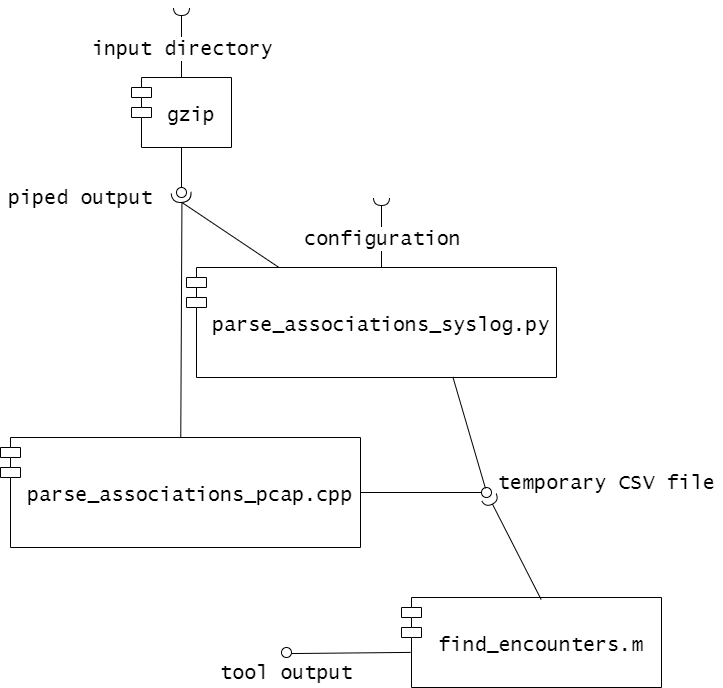
\includegraphics[width=0.8\textwidth]{component_diagram.png}
    \caption{This figure shows the different software components involved in the summarisation tool, and how they interface with each other. This is a high level representation of the system and shows no detail regarding how each component and interface works.}
    \label{fig:component_dia}
\end{figure}

Figure \ref{fig:component_dia} shows how the components of the summarisation tool are connected. There are separate association extraction components for each input type. As long as the correct interfaces are used for input and output it is a simple matter to connect a new program to parse and extract associations from a different input format.

\subsection{Stage One; Decompressing Files}

The datasets downloaded from the CRAWDAD site are initially compressed (as gzip files). A directory of compressed pcap files can be given as a parameter to the summarisation script. Each file in the given directory will be individually decompressed using gzip and piped into the first stage of the processing. This unfortunately causes associations which span multiple pcap files to be split at the temporal boundaries of the files.

\subsection{Stage Two; Extracting Associations}

Libpcap is a library written in C/C++ which provides functions for the analysis of network traffic, including reading and extracting information from pcap files such as those produced in tcpdump traces. Tcpdump was the utility used to capture the CRAWDAD dartmouth dataset on which this project is initially focused. There are several wrappers of libpcap written for different languages such as pycap \cite{pynetwork2019} for Python and jpcap \cite{charles2013}. These are generally not very regularly maintained and have very little documentation compared to Libpcap with C/C++. When initially reading in pcap files as input C++ will be used to extract the necessary information. In this stage of processing only information about the times of associations and MAC addresses of involved devices should be kept. Most of the processing will be done in subsequent stages, the main aim of this stage is to remove as much unnecessary information as possible, and to convert into an appropriate format for the next stage.

In this stage of processing a hash map of ongoing associations is built up during the reading of all packets from a pcap file. The map is updated every time a packet is read which signals the beginning of an association or the end of one. In the case of the beginning of an association, the map is updated by setting the MAC address pair to the two addresses between which the packet is sent (this is used as the key), and start and end times of the association are set to be the timestamp on the packet. Every time that a packet is read between a pair of devices the end time of the pairs current association is updated to the packets timestamp. Each packet is also checked to find whether the destination node of the pair is an access point. Since packet-specific information will be discarded after this stage it is necessary to identify access points with a flag. When the association ends, the values stored in the map are output in string delimited by commas. The values which are output are the source and destination MAC addresses, and start and end times of the association, and a flag (0 or 1) value identifying whether the destination device is an access point. This output is used as input in the subsequent processing stage.

\subsection{Stage Three; Finding Encounters} 

\begin{figure}[h]
    \centering
    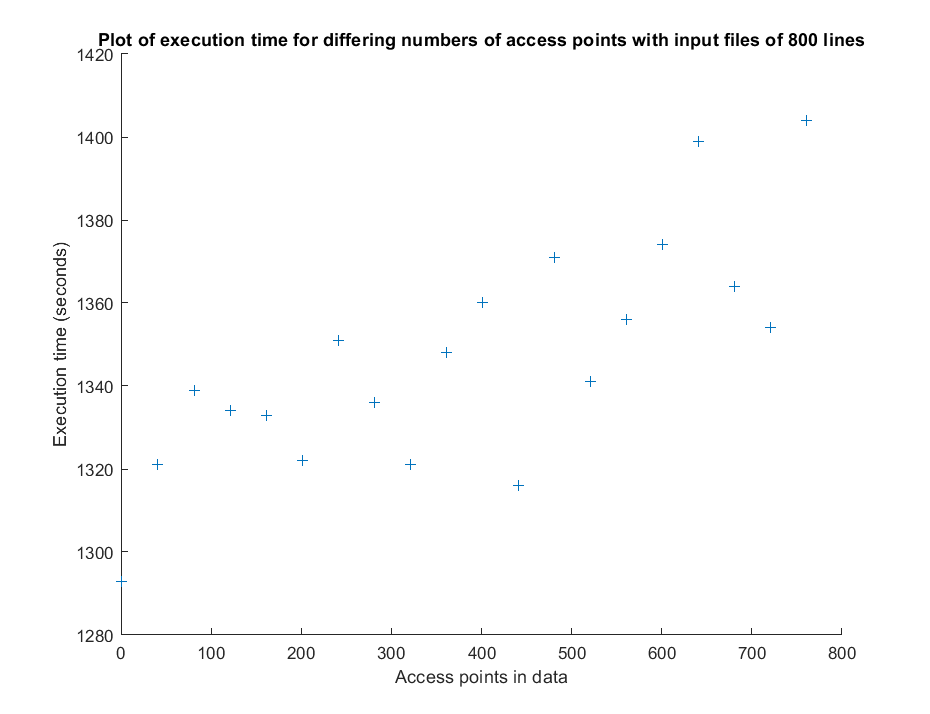
\includegraphics[width=\textwidth]{ap_vs_time.png}
    \caption{This figure shows the dependence of execution time on the number of access points in a file of associations for a file length of 800 lines. The files used as input to the MatLab code for this evaluation were fabricated to include specific numbers of distinct access point IDs. A roughly linear positive correlation is seen between the number of access points and the execution time.}
    \label{fig:AP_vs_time}
\end{figure}

The third stage of processing is written using MatLab. This decision was made due to the efficiency of the MatLab language when manipulating large tables of data (such as are used during this project) and my previous experience with the language in comparison to others similar such as Mathematica or Maple. Consideration was also given to continuing to develop this stage of processing using C++, similarly to the previous stage. This could potentially increase the efficiency and speed up processing time, however my familiarity with C++ is fairly limited and therefore the efficiency gained would likely not be worth the cost in development time by using C or C++.\\\\
This stage of processing has three main aims, firstly to extract a list of access points. Having a list of access points is important since encounters need to occur through access points (as described in the `Design' section). The second aim is to match up the timings of associations between mobile nodes and access points such that encounters can be identified. The final aim is to then find the average duration and frequency of encounters between each distinct pair of mobile nodes. 

\begin{figure}[h]
    \centering
    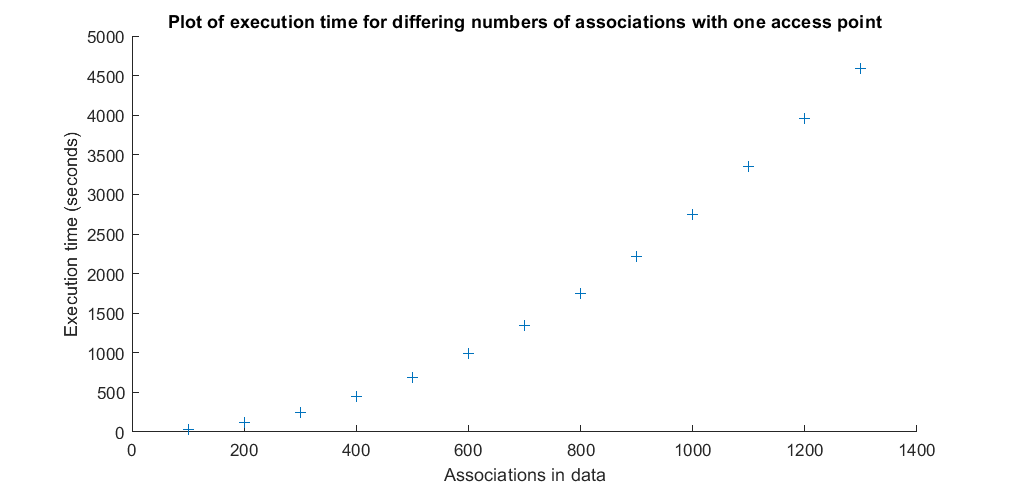
\includegraphics[width=\textwidth]{time_vs_lines.png}
    \caption{This figure shows the dependence of execution time on the number of associations in the intermediate file. Results are mean values averaged over ten iterations of each number of assciations. The files used as input to the MatLab code for this evaluation were fabricated to include specific numbers associations and a static number of access points. A power two positive correlation is seen between the number of associations and the execution time.}
    \label{fig:lines_vs_time}
\end{figure}

Initially the implementation of this stage of processing became drastically slower at high numbers of access points, this issue has been solved such that an almost linear behaviour in execution time if measured as the number of access points increases (shown in figure \ref{fig:AP_vs_time}) whereas in figure \ref{fig:lines_vs_time} it can be seen that the execution time still increases with a quadratic curve as the line length of the intermediate associations file increases. The limiting factor is now the total length of the input file for this stage of processing.



\section{Adjustments Due to CORVID-19}
\label{section:corvid}
%what you could not do
This project has not expected to use face-to-face user testing at any stage and, despite being written to run on the Linux lab machines in the School of Computer Science, all testing and development has been able to be completed remotely using ssh when necessary. No adjustments were made to the development or testing of this project as a direct consequence of the CORVID-19 virus.

A loss of working hours has resulted from the current circumstances due to having to move out of my flat at St Andrews, caring for elderly relatives, and other necessary engagements. However, the two week deadline extension has been sufficient to make up for any work lost during this upheaval.
%adjustments made
%additional time cost

\section{Evaluation and Critical Appraisal}
\label{section:eval}
The high priority requirements of this project have been met. There are several pieces of evidence and justification for this which will be discussed in the following paragraphs. One of the requirements was to reduces the quantity of data through summarising it, while maintaining useful information. The information in the final summaries produced has been chosen based on research into past studies completed using the CRAWDAD datasets. Key data which was used in the studies such as the encounters between devices, device identifications for the endpoints, and encounter duration are all present in the summary output. It can also be shown quantitatively that the quantity of data has been significantly reduced from the input data to the summarisation, figure \ref{fig:size_red} shows how the quantity of data is reduced for each building in the dartmouth/campus data. On average this is a reduction in the number of bytes of over 99\%. No relationship is seen between the initial size of the file and the size of the summary; there are a multitude of other factors at play determining the size reduction due to this test using real world data collected from various campus buildings and at differing times of year. \\\\
The main conclusion which can be drawn here is that the size of the input trace has less of an effect on the size of the output than the context in which the data was collected does. Consider hypothetically two data sets collected over the same period of time, one in a library and one in a student dormitory. Data collected from student dormitories is likely to produce large traces with a lot of traffic from applications such as streaming media, while the encounters in the building may be relatively few as only residents are likely to be present. In comparison to this, data collected from the library would be more likely to include far more users, and less traffic per user (the main network usage being more work orientated such as downloading academic papers and accessing lecture slides). From the two examples given here, it is clear that although the traffic in the dormitory may be similar or even higher than that of the library (determining the input data size), more encounters would be expected from the library data (determining the output summary size).

\begin{figure}[h]
    \centering
    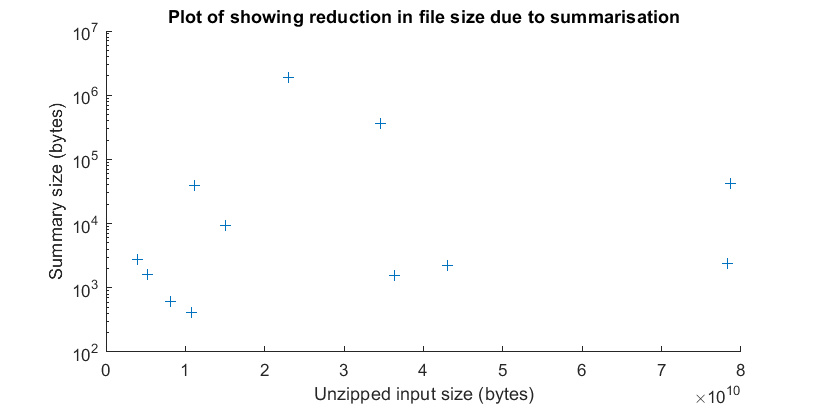
\includegraphics[width=\textwidth]{size_red.png}
    \caption{This figure shows the number of bytes in the unzipped input files compared to the bytes in the output file. This data was collected over the dartmouth/campus dataset where each input is the network trace of a specific campus building over a single measurement period. It can be seen that the number of bytes per files is reduced by between 3 and 8 orders of magnitude. This is a minimum reduction of 99.992\%.}
    \label{fig:size_red}
\end{figure}

This reduction in size also contributes somewhat to meeting the second requirement specified; the summary should be able to be processed more efficiently than the original data. Such a reduction in size denotes a reduction in the complexity and information content of the data. Assuming that the information required for further processing is still present in the summary, it will be much quicker to find in future processing tasks. In addition to this the default output of the tool is a simple CSV format, meaning that many tools and software packages will be compatible with it.
The final high priority requirement was that the output should use a common format which is appropriate to the context of this project. The use of specific data fields in the output are justified fully in section 3.2, the fields were chosen with consideration to past use of the dartmouth/campus datasets with the aim to include only information which was seen to be frequently relevant during previous research using the datasets. Although a CSV file could be argued to be a common format, it has little to no specific relevancy to the field of mobility research, requiring that specifically developed tools would need to be developed to further process the summaries produced by this project. That is why the option to output a summary of connection events was added. This events summary is compatible with the widely used ONE simulator \cite{Keranen2009}, a screenshot of the ONE simulator running on one of the produced events summaries is shown in figure \ref{fig:one} and an extract from a report produced from this simulation run is shown in figure \ref{fig:report}. A very basic settings file was used for the example simulation here, the values used and additional information which would be necessary for a realistic usage (such as connection speeds and geographical information) is out of scope of this project.
\begin{figure}[h]
    \centering
    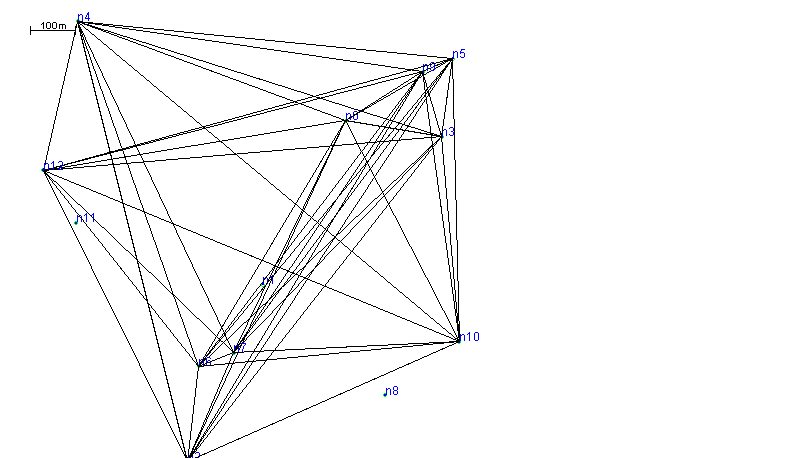
\includegraphics[width=\textwidth]{screenshot_one.png}
    \caption{This figure shows a still taken during the running of the ONE simuator using an events trace output by the summarisation tool developed in this project. The data input to the summarisation was an extract from the fall03 tcpdump dartmouth/campus \cite{dartmouthcampus2009} dataset}
    \label{fig:one}
\end{figure}
\begin{figure}[h]
    \centering
    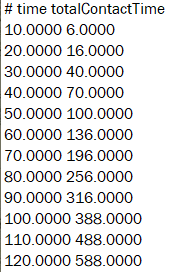
\includegraphics[width=0.3\textwidth]{contact_report.PNG}
    \caption{This figure shows an extract of the report (using TotalContactTimeReport) which was output from the run of the ONE simulator \cite{Keranen2009} shown in figure \ref{fig:one}}
    \label{fig:report}
\end{figure}

Summaries are able to be produced based on both syslog or tcpdump/pcap input files. The output produced using each input type is of the same format, however the format of the input needs to be specified at run time using an argument. This meets one of the medium priority requirements given earlier in this report and specified at the beginning of this project.

Unfortunately due to time restrictions no low priority requirements were able to be implemented. However it was kept in mind throughout development that adding further data formats to the input possibilities may become necessary (due to the low priority requirement of processing files of unknown input format), and this has influenced the structure of the system. The second stage of processing (extracting associations) is done within a separate software component for each different format, and adding a new component for a different input format would be trivial assuming it had been developed with the appropriate output format.

\section{Conclusions}
\label{section:conc}
The summarisation tool discussed in this document provides a way to convert multiple formats of collected network data into a single output format. This includes tcpdump network traces and syslog files (as long as some details of the syslog format are given). A brief summary of whether or not each project requirement has been fulfilled is given below. Each requirement is repeated here in bold as it was given initially in section \ref{section:req} for convenience.
\\\\
\textbf{Reduce the quantity of data from the original dataset while maintaining any information identified as useful during research into how CRAWDAD datasets are used.}
A significant reduction in the size of files has been observed when the summarisation tool is run on network traces collected from the campus buildings of Dartmouth College. The data regarding reduction in file size is displayed in figure \ref{fig:size_red}. In section \ref{section:useage} a through summary has been presented showing research into which information from the CRAWDAD data sets is most useful in the context of network mobility and DTNs. Using this research a default summary format, a comma separated encounter summary, has been specified.
\\\\
\textbf{Produce summaries of the initial datasets that can be processed more efficiently than the original data.}
A rather trivial point to make here is that by removing the unnecessary data from the raw network traces and reducing their size, the time taken to extract more specific information from the summary in future must be achievable in stricter time and memory limits. This is due to all searching and sorting algorithms being limited by the size of the input they take. 
This tool also allows multiple formats of input data to be converted to an identical output format. By implementing this feature it is possible that data collected from multiple sources may be processed using the same downstream systems. This could save researchers from needing to develop multiple downstream tools to handle different formats of input in cases where mixed methods of data capture might be used.
\\\\
\textbf{Use a commonly found format to output my summaries and justify why this format is appropriate in context.}
The tool offers an option to output the summary in the format of an events trace as used by the ONE simulator. The ONE simulator has been mentioned several times throughout this document, initially in the context survey where it was identified as a commonly used tool for studies around network mobility and DTNs. Providing this events format gives a link to an already widely used system in the area of network mobility, therefore allowing the summaries to be used without new downstream processing systems being developed.
\\\\
\textbf{Allow multiple summaries to be merged (this may allow extension into distributed processing).}
The merging tool developed during this project is documented in detail in section \ref{section:merge}. It allows for any number of summary files to be placed in a directory and merged together into a single summary of the same format. The input summaries must have the same format, and in the case of the ONE simulator compatible  event traces, a modified format must be used to create the summaries before the merge. If the normal event trace format is used, information will be lost and the files may not merge as intended.
Although no extension into distributed processing has been implemented, this possible use of the merging tool has been considered in section \ref{section:merge}.  
\\\\
\textbf{Summarise at least two different formats of input data to create a standard output summary.}
Initially network traces output by tcpdump were the input format this project was developed for use on, however this was extended to also take syslog files as input. In the case of syslog input there must be a configuration file with certain variables (such as the location and format of device identifications) given in addition to the input file. In both cases, tcpdump and syslog, the same output formats are available. 
\\\\
Unfortunately, due to the time constraints of this project the following three medium/low priority requirements were not able to be implemented:
\begin{itemize}
\item \textbf{Allow a summary to be updated by the addition of a single data entry (this may allow extension into real-time processing).}
\item \textbf{Process datasets with an unknown input format.}
\item \textbf{Identify and report if a specific summary is likely to be unrepresentative of the input dataset due to aspects such as missing data or bias.}
\end{itemize}

Despite these features not being implemented yet, future development has been considered throughout the project. The summarisation tool has been specifically designed to be easy to build on in terms of new input formats; only a small part of the system would need to be re-written for a new input type to be added to the system.
If the input data is comprised of a large number of zipped files (such as pcap files segmented by time like those in the Dartmouth dataset) the unzipping process can take a significant amount of time. However, this is unavoidable as the files cannot be processed while compressed. A large amount of input data can also lead to the third stage of processing taking a significant time to run, however this is determined by the number of associations and access points in the data and not by the total input size. These time dependencies have been taken into account during the development and have been minimised where possible. Specifically, the ability to process small chunks of the input data individually and then merge their summaries after they have been output from the tool would provide a quicker execution in some cases.\\\\

\newpage

\nocite{*}
\printbibliography

\appendix
\newpage
%\section{Appendix A: Testing Summary}
%\input{testing.tex}

%\section{Appendix B: User Manual}
%\input{manual.tex}

\section{Appendix A: Ethics Approval}
\label{section:ethics_append}

\includepdf[pages=-,pagecommand={},width=\textwidth]{Knight_ApprovalLetter[12798].pdf}

\end{document}
